\section{Introducción}
En esta sección se describe el proceso de investigación, que fue determinante a
la hora de definir la forma en que se iba a implementar la solución propuesta en
este trabajo.
En primer lugar se parte de una definición  prematura de los requerimientos y
objetivos. A partir de dicha definición se propone  una solución orientada a la
generación de código, y luego de la investigación se concluye en que una
solución basada en la creación de un framework es más apropiada para lograr el objetivo planteado.
\subsection{Aproximación de Requerimientos Inicial}
Con la intención de definir la orientación del trabajo, se realizó
una primera aproximación de la definición de los requerimientos y
objetivos.
Se toma como punto de partida el trabajo ~\cite{codegen}.

Una definición prematura del objetivo principal es:
``El sistema debe facilitar a desarrolladores de software la utilización de una
Red de Petri como motor lógico de su producto. Además debe obligar la
utilización de patrones de diseño en el código con el objetivo de reutilizar
diseños probados y robustos. \emph{\color{red}mejorar esto}''.
De manera análoga a la solución propuesta en ~\cite{codegen} la primer propuesta
de solución al problema planteado en este trabajo se basa en la generación de
código, añadiendo a dicha solución un enfoque orientado a la utilización patrones de diseño.
 En este sentido, se definen objetivos de investigación para determinar la
 factibilidad de desarrollo, idoneidad para cumplir el objetivo, mantenibilidad
 y escalabilidad de un sistema que cumpla con estas características. La investigación se centrara en los aspectos
 listados a continuación.
\begin{itemize}
    \item Determinar la posibilidad o imposibilidad de aplicar patrones de
    diseño mediante la generación de código fuente.
    \item Determinar la escalabilidad de generar código fuente para proyectos
    de software.
    \item Determinar la mantenibilidad del código fuente generado.
    \item Investigar la posibilidad de obligar la utilización de patrones
    de diseño en el código generado.
    \item Buscar otras alternativas de solución y compararlas con la generación
    de código.
\end{itemize}
Por otro lado, se realizó una definción aproximada de los primeros
requerimientos del sistema, basados en ~\cite{codegen} y en la propuesta
de utilización de patrones de diseño. A continuación son listados.
\begin{itemize}
    \item Capacidad de abrir y editar una red de Petri desde un archivo existente.
    \item Capacidad de guardar una red de Petri finalizada o en desarrollo.
    \item Utilizar un formato de archivo de red de Petri estándar.
    \item Definir el lenguaje a generar y su versión.
    \item El código generado deberá constar de: ”esqueletos” de procesos
    concurrentes definidos por el usuario (de manera que el usuario complete dichos esqueletos con el código secuencial de las funciones necesarias).
    \item Interfaz (API) que se comunique con el simulador de petri nets
    desarrollado en el Laboratorio de Arquitectura de Computadoras de la
    Universidad Nacional de Córdoba.
    \item Obtener un proyecto con los archivos generados por la herramienta
    (código fuente, archivos configuración, etc.), con formato que corresponda la lenguaje de programación elegido.
    \item Proveer al usuario de una interfaz gráfica para definir los procesos
    de su sistema. 
    \item Escribir un manual de uso y otro de especificaciones de la herramienta final.
    \item Proveer al usuario de una interfaz gráfica para definir la información
    de etiquetas de transición.
    \item Establecer una forma de relacionar las etiquetas de transición de la
    red con los procesos y métodos del sistema real.
    \item  Resolver problemas típicos de programación concurrente para poner a
    prueba el sistema.
\end{itemize}




\subsection{Nueva Definición de Requerimientos}
Basandonos en ~\cite{chimp}. A partir de nuestra primer prueba de concepto
\emph{\color{red} ANTES DE ESTO HAY QUE PONER LA INVESTIGACION DE PORQUE SE
DESCARTÓ LA GENERACIÓN DE CÓDIGO Y COMO LLEGAMOS A LA IDEA DE UN FRAMEWORK, ALGO
DEL DISEÑO DE LA PRIMER POC, LO DE LAS PLAZAS DE RECURSOS Y COMO SE REEMPLAZARON POR DISPAROS PERENNES}

\begin{enumerate}
	\item El sistema debe delegar flujo de ejecución a un motor de
	petri.
	\begin{itemize}
		\item El sistema debe mapear transiciones de una red de petri a eventos
		especificados por los usuarios. Un evento equivale a una
		conjunción de transiciones y guardas.
		\item Cuando un evento es desencadenado por el disparo de un conjunto de
		transiciones el sistema debe ejecutar todas las tareas que se encuentran registradas al evento.
		\item Cuando un suceso definido por el usuario ocurre, el sistema debe
		notificar todos los eventos asociados a este suceso al motor de petri.
		\item El sistema debe proveer una interface para que el usuario pueda
		suscribir sucesos, tareas y fines de tareas a eventos especificados por el usuario.
		\item El sistema debe proveer una interface para que el usuario pueda definir
		eventos.
		\item Cuando una tarea termina el sistema debe notificar al motor de petri
		acerca de todos los eventos asociados a la finalización de la tarea.
		%DEFINIMOS LA DIFERENCIA ENTRE SUCESO Y FIN DE TAREA CON LOS CASOS. DESDE EL
		%PUNTO DE VISTA DEL USUARIO ES DISTINTO, DESDE EL PUNTO DE VISTA DEL FRAMEWORK
		%EL FUNCIONAMIENTO ES IGUAL.
	\end{itemize}
	\item Para un usuario con conocimiento intermedio en Java y Redes de Petri, el
	framework puede aprender a usarse en una semana o menos.
	%VAMOS A MEDIR ESTE REQUERIMIENTO CON ALUMNOS DE LA CATEDRA PROGRAMACIÓN
	% CONCURRENTE DEL AÑO 2017
	\begin{itemize}
	    \item La utilización del sistema puede incorporar como máximo diez
	    conceptos nuevos a aprender por un usuario con un nivel intermedio en Java
	    y redes de Petri.
	    \item El sistema debe ser acompañado con al menos dos ejemplos de uso en
	    los cuales se muestre al menos un 80\% de las funciones del mismo.
	\end{itemize}
	\item El sistema debe ser compatible con las versiones actuales de motores de
	Petri desarrollados en el Laboratorio de Arquitectura de Computadoras de la
	Facultad de Ciencias Exactas y Naturales de la Universidad Nacional de Córdoba.
	\begin{itemize}
	    \item El sistema debe proveer una interfaz para que el usuario ingrese un
	    archivo PNML con la descripción de una red de Petri.
	    \item El sistema puede instanciar un entorno de ejecución de redes de
	    Petri dado que el usuario ha ingresado un archivo PNML conteniendo la
	    descripción de la red y ha elegido el motor de Petri que desea usar. 
	    %LOS MOTORES SON: JAVA, IPCORE Y DRIVER. EN ESTE TRABAJO VAMOS A ASEGURAR Y
	    % TESTEAR LA FUNCIONALIDAD CON EL MOTOR DE JAVA.
	    \item El sistema debe utilizar la interface expuesta por el motor de
	    petri.
	\end{itemize}
	
	
	\emph{\color{red} A PARTIR DE ESTE PUNTO SON TRABAJOS FUTUROS}

	\item El sistema quiere tener una interfaz gráfica de usuario para inicializar
	un nuevo proyecto.
	\begin{itemize}
	    \item La interfaz de usuario quiere contener una pantalla 'PNML Loader'
	    	\begin{itemize}
	    	    \item La pantalla debe dejar al usuario buscar en su disco local y
	    	    elegir un archivo.
	    	    \item La pantalla debe dejar al usuario ingresar la dirección a un
	    	    archivo manualmente mediante la escritura con el teclado.
	    	    \item La pantalla debe permitir confirmar la elección de un archivo.
	    	    \item Si el usuario confirma un archivo y el archivo es un PNML válido
	    	    entonces puede usarse para configurar el entorno de ejecución de
	    	    Petri.
	    	    \item Si el usuario confirma un archivo y el archivo no es un PNML
	    	    válido entonces debe mostrarse un error en pantalla y el usuario debe
	    	    ser capaz de elegir otro archivo.
	    	\end{itemize}
	    \item La interfaz de usuario quiere contener una pantalla de creación de
	    eventos
	    \begin{itemize}
	    	    \item La pantalla debe dejar al usuario definir un evento y asociarlo
	    	    con una o más transiciones definidas en un archivo PNML cargado
	    	    previamente por el usuario.
	    	    \item La pantalla de creación de eventos quiere permitir guardar las
	    	    decisiones del usuario en un archivo.
	    	    \item La pantalla de creación de eventos quiere permitir al usuario
	    	    cargar configuraciones a partir de un archivo.
	    	    \item Si un archivo guardado previamente se selecciona para ser
	    	    cargado y su contenido tiene un formato inválido, la pantalla
	    	    quiere mostrar un texto de error especificando el problema y el
	    	    archivo no debe ser cargado.
	    	    \item Si un archivo guardado previamente se selecciona para ser
	    	    cargado y el contenido del archivo contiene uno omás eventos que
	    	    mapean a transiciones inexistentes, la pantalla quiere mostrar un
	    	    texto de error especificando el problema y sólo debe cargarse la
	    	    configuración de los eventos fuera de conflicto.
	    \end{itemize}
	     \item La interfaz de usuario quiere contener una pantalla de selección de
	     el motor de Petri.
	     \begin{itemize}
	         \item La pantalla debe permitir elegir entre un motor de Petri Java,
	         un motor de Petri en hardware o un motor de Petri en driver.
	         \item La pantalla debe comunicar la decisión del usuario para preparar
	         el entorno de ejecución de Petri de acuerdo al motor elegido.
	     \end{itemize}
	         
	\end{itemize}
\end{enumerate}

Una vez definidos los nuevos requerimientos se procede a definir los casos de
uso mediante la utilización de un diagrama UML.


\begin{figure}[h]
    \centering
    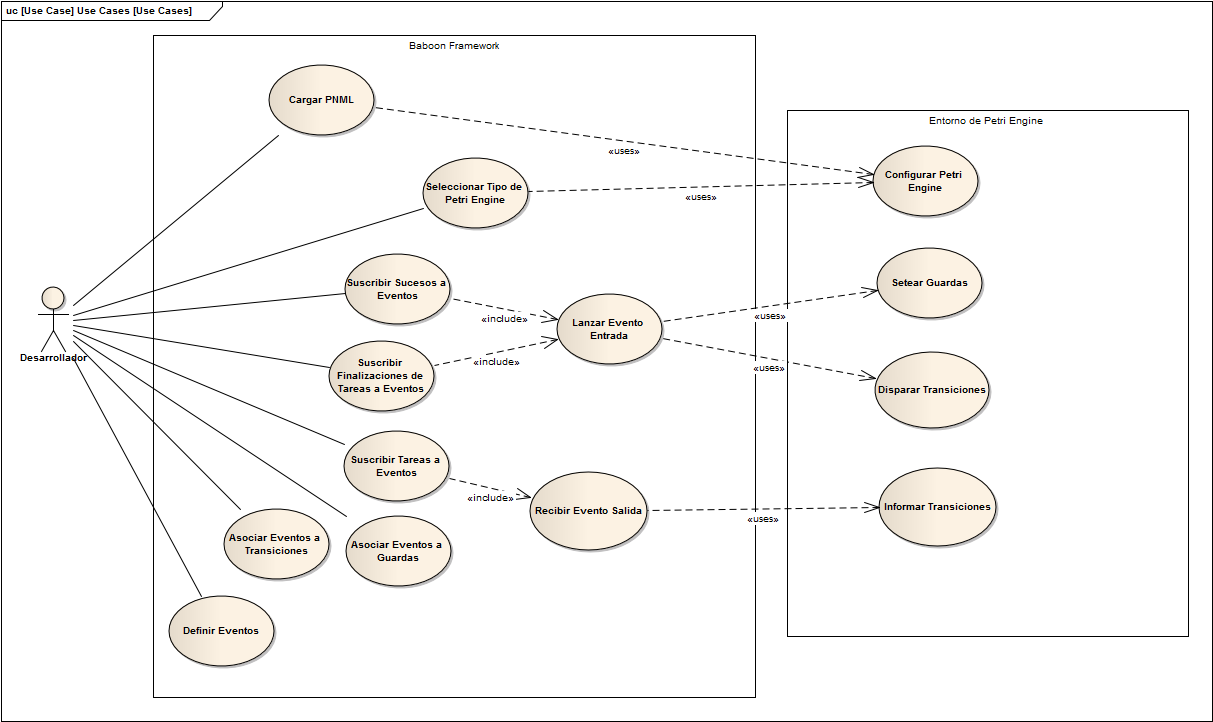
\includegraphics[width=\textwidth]{Use_Cases}
    \caption{Diagrama UML de Casos de Uso}
    \label{fig:casos_de_uso_uml}
\end{figure}

A partir de este diagrama se escriben los casos de uso de forma detallada. A
continuación se presentan los mismos.

\begin{itemize}
    \item ID: 001
    \begin{itemize}
        \item Nombre: Definir eventos
        \item Descripción: El usuario desarrollador de software del sistema debe
        poder definir eventos con un nombre de su elección.
       	\item Actor principal: Usuario desarrollador de software.
       	\item Precondiciones: 
       		\begin{itemize}
       		    \item Un archivo PNML válido ha sido cargado en el sistema.
   		    \end{itemize}
       	\item Flujo Básico: 
       		\begin{itemize}
       		    \item El usuario abre una interfaz gráfica dedicada a definir
       		    eventos y asociarlos a elementos de una red de petri.
       		    \item El usuario utiliza la herramienta para añadir un nuevo
       		    evento en la interfaz gráfica.
       		    \item El usuario debe nombrar el evento para poder definirlo. 
       		    \item Una vez nombrado, el usuario acepta el nombre y el nuevo
       		    evento queda definido.
       		    \item El usuario utiliza la herramienta para guardar los cambios.
       		    \item El usuario elige la ubicación y el nombre del archivo donde
       		    se guardaran los cambios.
       		    \item El usuario guarda los cambios y se crea un archivo
       		    conteniendo los eventos.
   		    \end{itemize}
	    \item Flujo Alternativo 1: 
           	\begin{itemize}
       		    \item El usuario abre una interfaz gráfica dedicada a definir
       		    eventos y asociarlos a una red de petri.
       		    \item El usuario añade un nuevo evento con un nombre en la interfáz
       		    gráfica.
       		    \item El usuario intenta añadir un segundo evento con el mismo
       		    nombre.
       		    \item Un error se muestra en pantalla y evita que el segundo evento
       		    sea definido. El usuario debe cambiar el nombre del segundo evento
       		    obligatoriamente.
       		    \item El usuario proporciona un nombre de evento que no ha
       		    sido utilizado previamente.
       		    \item El usuario acepta el nombre y el nuevo evento queda definido
       		    en la interfaz gráfica.
       		    \item El usuario utiliza la herramienta para guardar los cambios.
       		    \item El usuario elige la ubicación y el nombre del archivo donde
       		    se guardaran los cambios.
       		    \item El usuario guarda los cambios y se crea un archivo
       		    conteniendo los eventos
	    	\end{itemize}
	    \item Flujo Alternativo 2: 
           	\begin{itemize}
       		    \item El usuario abre una interfaz gráfica dedicada a definir
       		    eventos y asociarlos.
       		    \item El usuario utiliza la herramienta para cargar eventos
       		    previamente definidos.
       		    \item Los eventos definidos en una sesión anterior se muestran en
       		    la interfaz gráfica.
       		    \item El usuario añade un nuevo evento con un nombre de evento que no ha
       		    sido utilizado previamente.
       		    \item El usuario acepta el nombre y el nuevo evento queda definido
       		    en la interfaz gráfica.
       		    \item El usuario utiliza la herramienta para guardar los cambios.
       		    \item El usuario elige la ubicación y el nombre del archivo donde
       		    se guardaran los cambios.
       		    \item El usuario guarda los cambios y se escribe el archivo
       		    cargado previamente conteniendo los nuevos cambios.
	    	\end{itemize}
	    \item Flujo Alternativo 3:
	    	\begin{itemize}
       		    \item Precondiciones: Existe un evento en la interfaz gráfica.       		  
       		    \item El usuario selecciona el evento existente en la interfaz
       		    gráfica y utiliza la herramienta de edición de eventos.
       		    \item El usuario elige un nuevo nombre para el evento distinto al
       		    que tenía previamente.
       		    \item El usuario acepta el nuevo nombre y el evento queda
       		    re-definido en la interfaz gráfica.
       		    \item El usuario utiliza la herramienta para guardar los cambios.
       		    \item El usuario elige la ubicación y el nombre del archivo donde
       		    se guardaran los cambios.
       		    \item El usuario guarda los cambios y se escribe el archivo de
       		    eventos.
	    	\end{itemize}
	    \item Flujo Alternativo 4:
	    	\begin{itemize}
       		    \item Precondiciones: Existe un evento en la interfaz gráfica.       		  
       		    \item El usuario selecciona el evento existente en la interfaz
       		    gráfica y utiliza la herramienta de eliminación de eventos.
       		    \item El evento desaparece de la interfaz gráfica y su nombre ahora
       		    puede utilizarse para crear un nuevo evento.
       		    \item El usuario utiliza la herramienta para guardar los cambios.
       		    \item El usuario elige la ubicación y el nombre del archivo donde
       		    se guardaran los cambios.
       		    \item El usuario guarda los cambios y se escribe el archivo de
       		    eventos.
	    	\end{itemize}
	    \item Flujo Alternativo 5:
	    	\begin{itemize}
	    	    \item El usuario abre la interfaz gráfica de eventos.
	    	    \item El usuario crea un evento nuevo.
	    	    \item El usuario cierra la interfaz gráfica sin guardar los cambios
	    	    \item La interfaz gráfica muestra un cartel preguntando al usuario si
	    	    desea guardar los cambios.
	    	    \item El usuario selecciona salir sin guardar cambios
	    	    \item La interfaz se cierra y no se escribe ni se sobreescribe ningún
	    	    archivo.
	    	\end{itemize}
	    \item Postcondiciones:
	    	\begin{itemize}
	       	    \item Un archivo conteniendo la definición de los eventos es
	       	    creado y guardado en disco.
	       	\end{itemize}
    \end{itemize}
    
    
    \item ID: 002
    \begin{itemize}
        \item Nombre: Asociar eventos a transiciones y guardas
        \item Descripción: El usuario desarrollador de software debe poder
        asociar eventos a un conjunto de transiciones y/o guardas.
       	\item Actor principal: Usuario desarrollador de software
       	\item Precondiciones: 
       		\begin{itemize}
       		    \item Un archivo PNML válido ha sido cargado en el sistema.
   		    \end{itemize}
    	\item Flujo Básico: 
       		\begin{itemize}
       		    \item El usuario abre la interfaz gráfica dedicada a crear eventos
       		    y asociarlos a elementos de la red de petri.
       		    \item La interfaz gráfica muestra al usuario una lista de las
       		    transiciones y guardas disponibles en la red de petri especificada
       		    en el archivo pnml.
       		    \item El usuario crea un nuevo evento asignandole un nombre.
       		    \item El usuario asigna a dicho evento un conjunto de
       		    transiciones informadas, las transiciones disparadas y las
       		    guardas que afecta (y su valor, verdadero o falso) utilizando un elemento de la
       		    interfaz gráfica asociado al evento creado. Todos los eventos
       		    deben tener asociado un elemento que permite realizar esta acción.
       		    \item El usuario utiliza la herramienta para guardar los cambios.
       		    \item El usuario elige la ubicación y el nombre del archivo donde
       		    se guardaran los cambios.
       		    \item El usuario guarda los cambios y se escribe el archivo de
       		    eventos conteniendo toda la información de los eventos y sus
       		    asociaciones.
   		    \end{itemize}
       	\item Flujo Alternativo 1: 
       		\begin{itemize}
       		    \item  Precondicion: Un archivo de eventos con asociaciones existe
       		    en el sistema.
       		    \item El usuario abre la interfaz gráfica dedicada a crear eventos
       		    y asociarlos a elementos de la red de petri.
       		    \item El usuario carga el archivo de asociaciones de eventos desde
       		    el disco.
       		    \item El archivo tiene un formato inválido.
       		    \item La interfaz gráfica muestra un error en pantalla.
       		    \item La interfaz gráfica No muestra los eventos del archivo. 
       		    \item La interfaz gráfica permite cargar otro archivo y/o definir
       		    los eventos manualmente.
       		    \item El usuario define nuevas asociaciones
       		    eventos-transición o eventos-guarda válidas
       		    \item El usuario utiliza la herramienta para guardar los cambios.
       		    \item El usuario elige la ubicación y el nombre del archivo donde
       		    se guardaran los cambios.
       		    \item El usuario guarda los cambios y se escribe el archivo de
       		    eventos conteniendo toda la información de los eventos y sus
       		    asociaciones.
   		    \end{itemize}
       	\item Flujo Alternativo 2: 
       		\begin{itemize}
       		    \item  Precondicion: Un archivo de eventos con asociaciones existe
       		    en el sistema.
       		    \item Precondicion: Se carga en el sistema un segundo archivo PNML
       		    con cambios respecto al original.
       		    \item El usuario abre la interfaz gráfica dedicada a crear eventos
       		    y asociarlos a elementos de la red de petri.
       		    \item El usuario carga el archivo de asociaciones de eventos desde
       		    el disco.
       		    \item El archivo tiene formato válido
       		    \item El archivo contiene asociaciones a transiciones y/o guardas
       		    que no se encuentran disponibles en el nuevo archivo pnml.
       		    \item La interfaz muestra un error en pantalla
       		    \item La interfaz gráfica muestra en pantalla sólo las asociaciones válidas.
       		    \item La interfaz permite asociar los eventos existentes o nuevos
       		    eventos a las transiciones y guardas de la nueva red.
       		    \item El usuario utiliza la herramienta para guardar los cambios.
       		    \item El usuario elige la ubicación y el nombre del archivo donde
       		    se guardaran los cambios.
       		    \item El usuario guarda los cambios y se escribe el archivo de
       		    eventos conteniendo toda la información de los eventos y sus
       		    asociaciones.
   		    \end{itemize}
       	\item Postcondiciones: 
       		\begin{itemize}
       		    \item Un archivo conteniendo la definición de los eventos y sus
       		    asociaciones con transiciones y guardases creado y guardado en
       		    disco.
   		    \end{itemize} 		  
    \end{itemize}
    
    \item ID: 003
    \begin{itemize}
        \item Nombre: Suscribir tareas y finalizaciones de tarea a
        eventos especificos
        \item Descripción: El usuario debe ser capaz de suscribir las tareas de
        software desarrolladas y sus finalizaciones, en caso de ser necesario, a
        los eventos del framework especificados.
       	\item Actor principal: Usuario desarrollador de software
       	\item Precondiciones: 
       		\begin{itemize}
       		    \item Se ha definido  un evento \{E1\} y se ha asociado a un
       		    conjunto de transiciones informadas, de transiciones disparadas y de guardas.
   		    \end{itemize}
    	\item Flujo Básico: 
       		\begin{itemize}
       		    \item El usuario utiliza una interfaz del framework que permite
       		    asociar una tarea o suceso específico a un evento específico
       		    \{E1\}.
       		    \item El usuario provee a la interfaz del framework un descriptor
       		    de la tarea y un descriptor del evento.
       		    \item Ambos descriptores son válidos y correctos.
       		    \item El flujo de ejecución de la tarea se delega al
       		    framework.
   		    \end{itemize}
       	\item Flujo Alternativo 1: 
       		\begin{itemize}
       		    \item El usuario utiliza una interfaz del framework que permite
       		    asociar una tarea o suceso específico a un evento específico
       		    \{E1\}.
       		    \item El usuario provee a la interfaz del framework un descriptor
       		    de la tarea y un descriptor del evento.
       		    \item El descriptor de la tarea es inválido.
       		    \item Al inicializar el framework ocurre un error crítico en tiempo
       		    de ejecución.
       		    \item Se guarda la descripción del error en un archivo log.
   		    \end{itemize}
       	\item Flujo Alternativo 2: 
       		\begin{itemize}
       		    \item El usuario utiliza una interfaz del framework que permite
       		    asociar una tarea o suceso específico a un evento específico
       		    \{E1\}.
       		    \item El usuario provee a la interfaz del framework un descriptor
       		    de la tarea y un descriptor del evento.
       		    \item El descriptor del evento \{E1\} es inválido.
       		    \item Al inicializar el framework ocurre un error crítico en tiempo
       		    de ejecución.
       		    \item Se guarda la descripción del error en un archivo log.
   		    \end{itemize}
       	\item Postcondiciones: 
       		\begin{itemize}
       		    \item  El flujo de ejecución de la tarea se delega al
       		    framework. Si existe un error de suscripción se genera un error en
       		    tiempo de ejecución y se guarda en un log.
   		    \end{itemize} 		  
    \end{itemize}

\end{itemize}

\begin{itemize}
    \item ID: TEMPLATE
    \begin{itemize}
        \item Nombre:
        \item Descripción: 
       	\item Actor principal: 
       	\item Precondiciones: 
       		\begin{itemize}
       		    \item 
   		    \end{itemize}
    	\item Flujo Básico: 
       		\begin{itemize}
       		    \item 
   		    \end{itemize}
       	\item Flujo Alternativo 1: 
       		\begin{itemize}
       		    \item 
   		    \end{itemize}
       	\item Flujo Alternativo 2: 
       		\begin{itemize}
       		    \item 
   		    \end{itemize}
       	\item Postcondiciones: 
       		\begin{itemize}
       		    \item 
   		    \end{itemize} 		  
    \end{itemize}
\end{itemize}
